\documentclass[tikz,border=10pt]{standalone}
\usepackage{tikz}
\usetikzlibrary{calc,angles,quotes}
\usepackage{fontspec}
\setmainfont{Khmer OS Battambang}
\definecolor{brandNavy}{RGB}{20, 45, 95}
\definecolor{brandCrimson}{RGB}{185, 25, 40}
\definecolor{brandTealBg}{RGB}{238, 246, 248}

\begin{document}
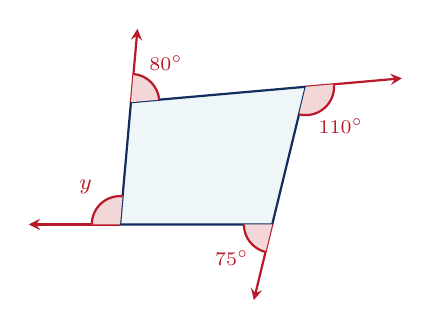
\begin{tikzpicture}[scale=1.15]
  \coordinate (D) at (0, 0);
  \coordinate (A) at (0.12, 1.35);
  \coordinate (B) at (2.05, 1.52);
  \coordinate (C) at (1.68, 0);

  % Polygon Fill and Outline
  \fill[brandTealBg] (A) -- (B) -- (C) -- (D) -- cycle;
  \draw[thick, brandNavy] (A) -- (B) -- (C) -- (D) -- cycle;

  % Extension coordinates
  \coordinate (XA) at ($(D)!1.6!(A)$);
  \coordinate (XB) at ($(A)!1.55!(B)$);
  \coordinate (XC) at ($(B)!1.55!(C)$);
  \coordinate (XD) at ($(C)!1.6!(D)$);

  % Extension Rays with Arrows
  \draw[thick, brandCrimson, ->, >=stealth] (A) -- (XA);
  \draw[thick, brandCrimson, ->, >=stealth] (B) -- (XB);
  \draw[thick, brandCrimson, ->, >=stealth] (C) -- (XC);
  \draw[thick, brandCrimson, ->, >=stealth] (D) -- (XD);

  % Angle Arcs (exterior angle sectors)
  \pic [draw, brandCrimson, thick, fill=brandCrimson!18, angle radius=0.36cm] {angle = B--A--XA};
  \pic [draw, brandCrimson, thick, fill=brandCrimson!18, angle radius=0.36cm] {angle = C--B--XB};
  \pic [draw, brandCrimson, thick, fill=brandCrimson!18, angle radius=0.36cm] {angle = D--C--XC};
  \pic [draw, brandCrimson, thick, fill=brandCrimson!18, angle radius=0.36cm] {angle = A--D--XD};

  % Labels placed EXACTLY in the exterior angle sectors:
  % 1. At A: sector between AB (east) and XA (north) -> bisector ~ 45 deg
  \node[font=\fontsize{7.5}{7.5}\selectfont\bfseries, color=brandCrimson] at ($(A)+(48:0.58cm)$) {$80^\circ$};

  % 2. At B: sector between XB (east) and BC (south-south-west) -> bisector ~ -50 deg
  \node[font=\fontsize{7.5}{7.5}\selectfont\bfseries, color=brandCrimson] at ($(B)+(-48:0.58cm)$) {$110^\circ$};

  % 3. At C: sector between XC (south-south-west) and CD (west) -> bisector ~ 218 deg
  \node[font=\fontsize{7.5}{7.5}\selectfont\bfseries, color=brandCrimson] at ($(C)+(220:0.58cm)$) {$75^\circ$};

  % 4. At D: sector between XD (west) and DA (north) -> bisector ~ 133 deg
  \node[font=\fontsize{8.5}{8.5}\selectfont\bfseries, color=brandCrimson] at ($(D)+(133:0.56cm)$) {$y$};
\end{tikzpicture}
\end{document}
